\chapter{Fondamenti Teorici}\label{fondamenti_teorici}

Questa sezione è dedicata a ricapitolare in breve le nozioni teoriche dell'ottimizzazione lineare che verranno applicate al problema del TSP. Inoltre, saranno fatte delle prime considerazioni sul problema del TSP con alcuni concetti sulla modalità di rappresentazione tramite grafi. Le formulazioni usate per la risoluzione del problema verranno trattate nel capitolo successivo.

\section{Ottimizzazione lineare}

L'ottimizzazione lineare è una branca dell'ottimizzazione matematica che si occupa di risolvere problemi di massimizzazione o minimizzazione di una funzione lineare soggetta a un insieme di vincoli lineari. Un problema di ottimizzazione lineare può essere espresso nel seguente formato:


\begin{math}
\text{minimize} \quad c_1 x_1 + c_2 x_2 + \ldots + c_n x_n
\end{math}

\begin{math}
\begin{aligned}
& \text{subject to} \\
& a_{11} x_1 + a_{12} x_2 + \ldots + a_{1n} x_n \geq b_1 \\
& a_{21} x_1 + a_{22} x_2 + \ldots + a_{2n} x_n \geq b_2 \\
& \quad \vdots \\
& a_{m1} x_1 + a_{m2} x_2 + \ldots + a_{mn} x_n \geq b_m \\
\end{aligned}
\end{math}



\begin{math}
 x_1 \geq 0, \quad x_2 \geq 0, \quad \ldots, \quad x_n \geq 0
\end{math}


dove \begin{math}c_1, c_2, ..., c_n \end{math} 
sono i coefficienti dei costi per le variabili decisionali \begin{math}x_1, x_2, ..., x_n \end{math}. \begin{math}a_{1_1}, a_{1_2}, ..., a_{m_n} \end{math} 
sono i coefficienti dei vincoli tecnologici, mentre 
\begin{math}b_1, b_2, ..., b_m \end{math}
sono i termini noti.

Durante il corso abbiamo visto che certi problemi di PL richiedono che le  variabili decisionali assumano valori interi. In tal caso, lo spazio ammissibile è l'insieme dei punti a coordinate intere. Nel caso del Problema del commesso viaggiatore si ha una situazione simile in quanto nelle formulazioni che tratteremo le variabili decisionali assumono valori booleani.


\section{Introduzione ai Grafi}
Un grafo è una struttura dati che rappresenta un insieme di oggetti, chiamati nodi o vertici, collegati tra loro da archi. I grafi sono usati per modellare e analizzare relazioni tra elementi di un insieme e sono ampiamente utilizzati in svariati campi. Spesso vengono rappresentati come \textit{G = (V, E)} dove V è l'insieme dei nodi ed E è una famiglia di coppie di elementi di V che rappresentano i collegamenti tra i nodi.

\subsection{Tipologie}
Ci sono diverse tipologie di grafi, tra cui grafi non orientati, grafi orientati e grafi pesati \cite{fischetti}.

\begin{figure}[ht]
	\centering
	\begin{minipage}[b]{0.3\linewidth}
		\centering
		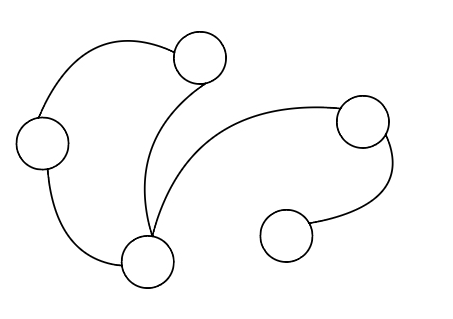
\includegraphics[width=\linewidth]{images/graf_non_orient}
		\caption{\textit{Esempio grafo non orientato}}
		\label{img:graf_non_orient}
	\end{minipage}
	\hfill
	\begin{minipage}[b]{0.3\linewidth}
		\centering
		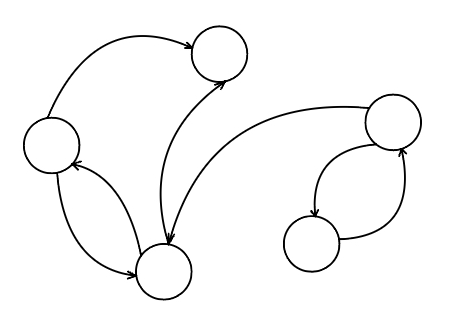
\includegraphics[width=\linewidth]{images/graf_orient}
		\caption{\textit{Esempio grafo orientato}}
		\label{img:graf_orient}
	\end{minipage}
	\hfill
	\begin{minipage}[b]{0.3\linewidth}
		\centering
		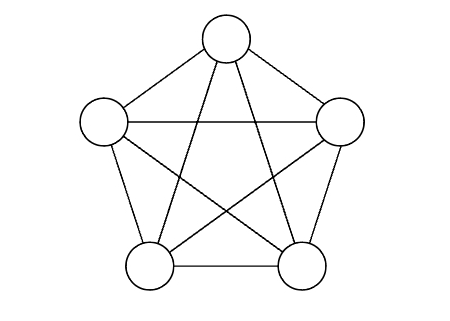
\includegraphics[width=\linewidth]{images/graf_complet}
		\caption{\textit{Esempio grafo completo non orientato}}
		\label{img:graf_complet}
	\end{minipage}
\end{figure}

\begin{itemize}
    \item nei \textbf{Grafi non Orientati} gli archi non hanno una direzione specifica; pertanto, una connessione tra due nodi è rappresentata da un arco che collega i due nodi senza una distinzione tra nodo di partenza e nodo di arrivo. 

    \item nei \textbf{Grafi Orientati} gli archi hanno una direzione specifica; quindi, una connessione tra due nodi è rappresentata da un arco diretto che ha origine da un nodo di partenza e finisce in un nodo di arrivo. Ad esempio, un grafo orientato può rappresentare una rete di collegamenti ipertestuali tra le pagine web, in cui i nodi sono le pagine e gli archi indicano i collegamenti da una pagina all'altra.

    \item nei \textbf{Grafi Completi} si ha un grafo non orientato in cui vi è un arco tra ogni coppia di nodi. In altre parole, ogni nodo è direttamente collegato a tutti gli altri nodi del grafo.

    \item nei \textbf{Grafi Pesati} a ciascun arco viene assegnato un valore o un peso che rappresenta qualche tipo di attributo o costo associato all'arco. Ad esempio, un grafo pesato può rappresentare una rete stradale in cui i nodi sono intersezioni, gli archi sono le strade e i pesi associati indicano il tempo di percorrenza di una determinata strada.
\end{itemize}

\subsection{Cammini}
Ci sono varie nozioni riguardanti i grafi. Per la nostra tesina e la successiva analisi del TSP, riteniamo utile introdurre quelli relativi ai cammini. 

Un \textit{cammino} di un grafo \textit{G = (V, E)} è una sequenza di archi consecutivi i quali permettono di collegare due vertici di V visitando una sequenza di vertici intermedi. 

Il vertice appartenente ad un grafo si dice \textit{connesso} ad un altro vertice dello stesso grafo semplicemente se esiste un cammino che collega i due vertici.

Se nel cammino il vertice di arrivo è uguale a quello di partenza si ha un \textit{ciclo}. 

Un ciclo semplice si dice \textit{Hamiltoniano} se visita una ed una sola volta tutti i vertici del grafo.

\begin{figure}[ht]
	\centering
	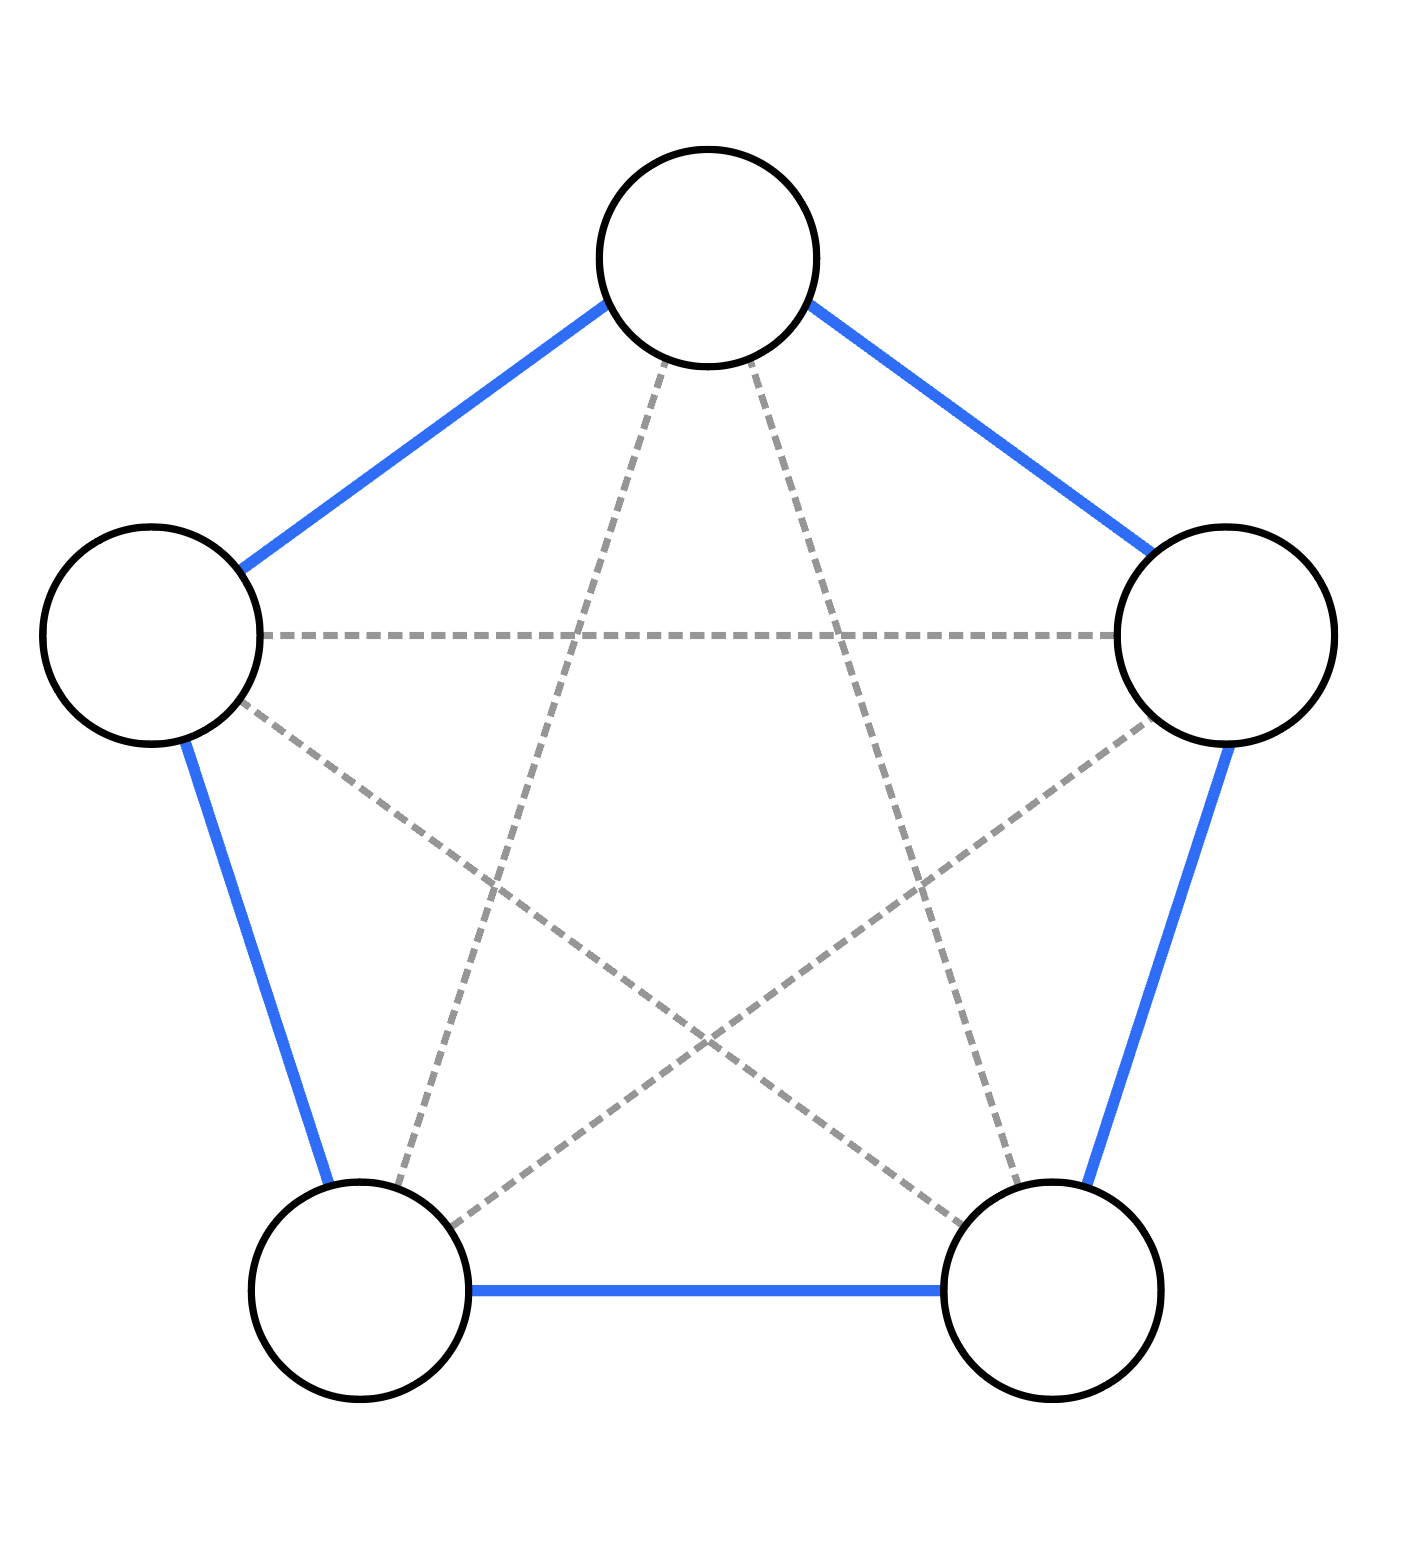
\includegraphics[width=.4\columnwidth]{images/es_ciclo_hamiltoniano}
	\caption{\textit{Esempio Cammino Hamiltoniano}}
	\label{img:es_ciclo_hamiltoniano}
\end{figure}

Possiamo ora riformulare il problema del TSP come: dato un grafo \textit{G = (V, E)} con dei pesi associati ad ogni arco, si cerca di individuare un ciclo hamiltoniano di costo minimo.

Possiamo fare una prima considerazione per il \textit{Problema del Commesso Viaggiatore} in relazione al numero dei cicli che si possono avere.

\subsection{Numero di cicli}
In un grafo completo con n nodi, ogni permutazione dei nodi forma un ciclo hamiltoniano. Poiché ci sono n nodi, ci sono n! permutazioni possibili. Tuttavia, poiché un ciclo hamiltoniano può essere percorso in entrambe le direzioni, ogni ciclo hamiltoniano viene contato due volte (una volta in senso orario e una volta in senso antiorario). Siccome abbiamo un numero fattoriale di potenziali soluzioni da esplorare, enumerare tutte le potenziali soluzioni sembra proprio una cattiva idea.
